\documentclass[12pt,a4paper]{article}
\usepackage[utf8]{inputenc}
\usepackage[T1]{fontenc}
\usepackage[portuguese]{babel}
\usepackage{graphicx}
\usepackage{float}
\usepackage{geometry}
\usepackage{amsmath}
\usepackage{booktabs}
\geometry{a4paper, margin=2.5cm}

\title{\textbf{Relatório Final: Controle de Aeropêndulo com NMPC Aproximado via Rede Neural}}
\author{Felipe Eduardo Marcondes}
\date{\today}

\begin{document}

\maketitle

\section{Introdução e Contexto}

Este relatório documenta a validação experimental e o desenvolvimento de um controlador neural embarcado para o rastreamento angular de um aeropêndulo instrumentado. O objetivo do projeto foi contornar o elevado custo computacional do Controle Preditivo Não-Linear (NMPC) tradicional em microcontroladores de baixo custo (STM32F446RE), executando as inferências de uma Rede Neural do tipo Multilayer Perceptron (MLP) treinada para imitar a lei de controle ótima. 

O sistema físico consiste em um motor Brushless (BLDC) monitorado por uma IMU (ICM-20948), cuja dinâmica de transição e posicionamento exigiu soluções avançadas em relação ao controle PID padrão, dados seus componentes não-lineares, principalmente o torque aerodinâmico e a gravidade pendular.

\section{Metodologia}

O desenvolvimento seguiu três fases principais, unindo identificação de sistemas baseada em dados, otimização preditiva e aprendizado de máquina embarcado:

\begin{enumerate}
    \item \textbf{Identificação do Modelo Dinâmico (NARX)}: Devido às não-linearidades do empuxo e aos atritos complexos do mancal, optou-se por modelar a planta utilizando o modelo fenomenológico NARX (Non-linear Autoregressive Network with Exogenous Inputs). Sinais de excitação diversos, incluindo variações de degraus, \textit{swept sines} e multissenos (com fases aleatórias), foram injetados na malha de um controlador PID base para capturar toda a dinâmica operacional. A validação demonstrou que o modelo previu as saídas do aeropêndulo com notável precisão (\textit{free-run}).
    
    \item \textbf{Formulação e Síntese do Controlador MPC}: De posse do modelo NARX, o Problema de Controle Ótimo (OCP) foi construído e solucionado de modo \textit{offline} através da biblioteca CasADi em linguagem Python. Diversos sinais de referências (como degraus variados, rampas e multissenos) foram expostos ao otimizador para a construção de um denso conjunto de dados (\textit{dataset}). Esse \textit{dataset} foi concebido para correlacionar o estado temporal do rastreamento à ação ideal (ótima) do atuador.
    
    \item \textbf{Aproximação Neural e Embarque (TinyML)}: Uma rede neural do tipo MLP, configurada com funções de ativação \textit{ReLU} (compatíveis com as funções afins por partes do EMPC), foi treinada \textit{offline} em PyTorch visando minimizar o Erro Quadrático Médio (MSE) entre as suas saídas e as ações calculadas pelo controlador ótimo original. O modelo treinado foi quantizado/compilado diretamente em um código C nativo por meio de uma matriz de pesos (\texttt{ann\_weights.h}) leve e performática, permitindo latências restritas de processamento inferiores aos 10 ms estabelecidos pelo projeto.
\end{enumerate}

\section{Resultados e Validação Experimental}

O projeto estruturou uma tríade de validação rigorosa, comparando as inferências nos ambientes:
\begin{itemize}
    \item \textbf{Python}: Simulador CasADi + MLP em PyTorch.
    \item \textbf{SIL (Software-in-the-Loop)}: Simulando o ambiente restrito com parâmetros nativos em C.
    \item \textbf{Real (Bancada Física)}: Embarcado no STM32 atuando na gravidade e aerodinâmica real.
\end{itemize}

Foram rodadas três principais baterias de sinais de validação. A Tabela \ref{tab:rmse} ilustra a fidelidade e estabilidade do rastreamento.

\begin{table}[H]
    \centering
    \caption{Tabela Comparativa de Desempenho (Raiz do Erro Quadrático Médio - RMSE)}
    \label{tab:rmse}
    \begin{tabular}{@{}lccc@{}}
        \toprule
        \textbf{Teste Realizado} & \textbf{Python} & \textbf{SIL (STM32)} & \textbf{Real (Bancada)} \\ \midrule
        Validação Principal (Multisseno + Degraus) & 1.56$^\circ$ & 2.85$^\circ$ & 3.26$^\circ$ \\
        Validação 2 (Degraus Aleatórios)           & 4.31$^\circ$ & 4.63$^\circ$ & 4.77$^\circ$ \\
        Validação 3 (Senoidal Suave)               & 1.37$^\circ$ & 1.50$^\circ$ & 3.01$^\circ$ \\ \bottomrule
    \end{tabular}
\end{table}

O desempenho se manteve consistente nos três ambientes de simulação e execução, apontando um sucesso massivo do transporte do MPC para o modelo polinomial embarcado via regressão neural.

\subsection{Gráficos e Comportamento dos Sinais}

As imagens a seguir evidenciam o esforço do controlador e a posição angular resultante para a Rede Neural atuando nas diferentes baterias de sinal.

\begin{figure}[H]
    \centering
    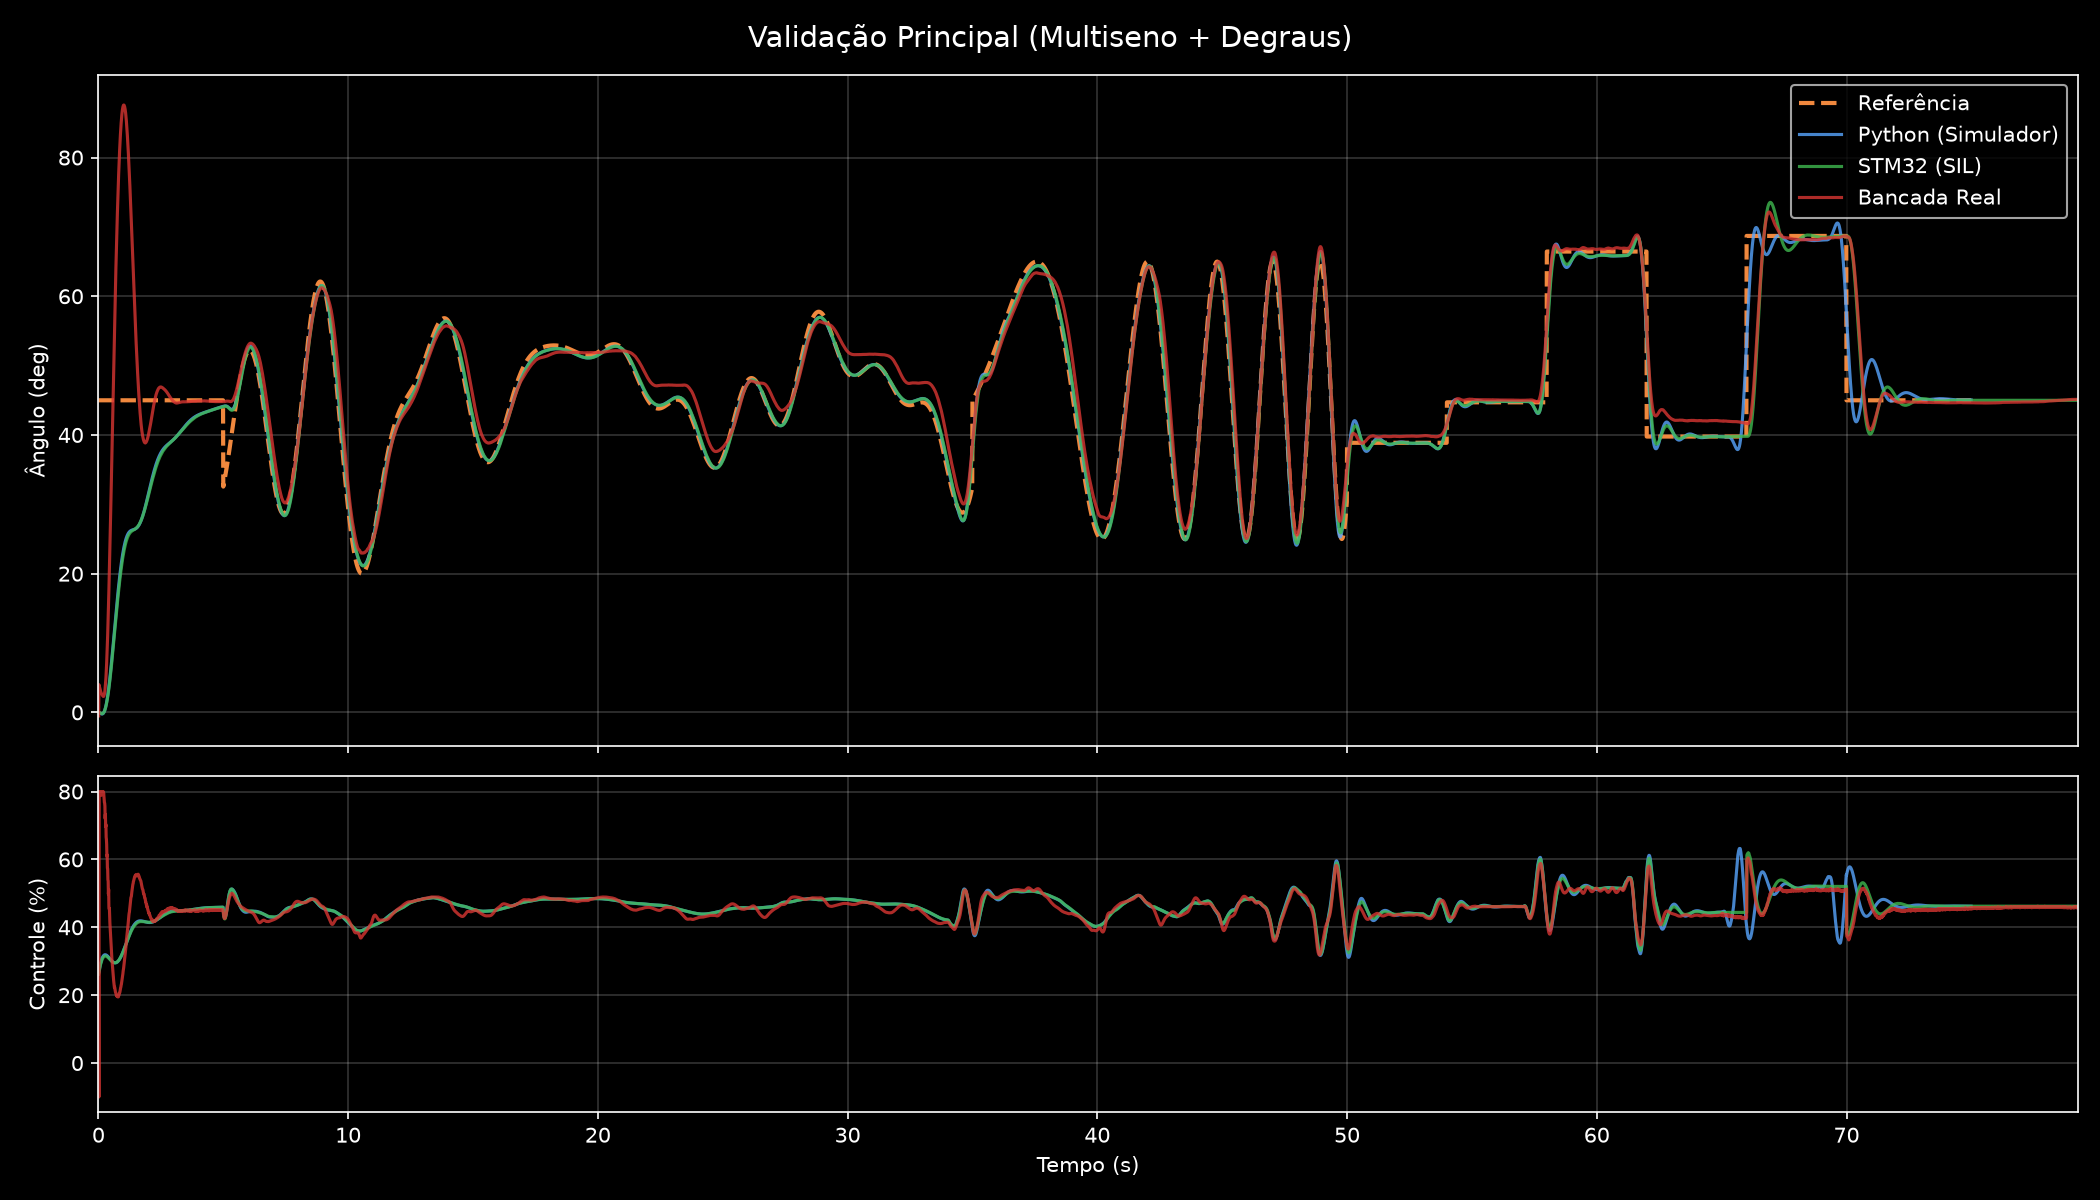
\includegraphics[width=0.95\textwidth]{imagens/comparacao_plot_0.png}
    \caption{Validação Principal (Multisseno + Degraus).}
    \label{fig:val1}
\end{figure}
Neste teste, as referências ágeis demonstraram leve \textit{delay} de transporte na bancada física em relação ao SIL, algo perfeitamente aceitável e originado possivelmente por efeitos de histerese eletromecânica no controlador ESC ou no motor que não foram mapeados de forma agressiva no espaço amostral do NARX.

\begin{figure}[H]
    \centering
    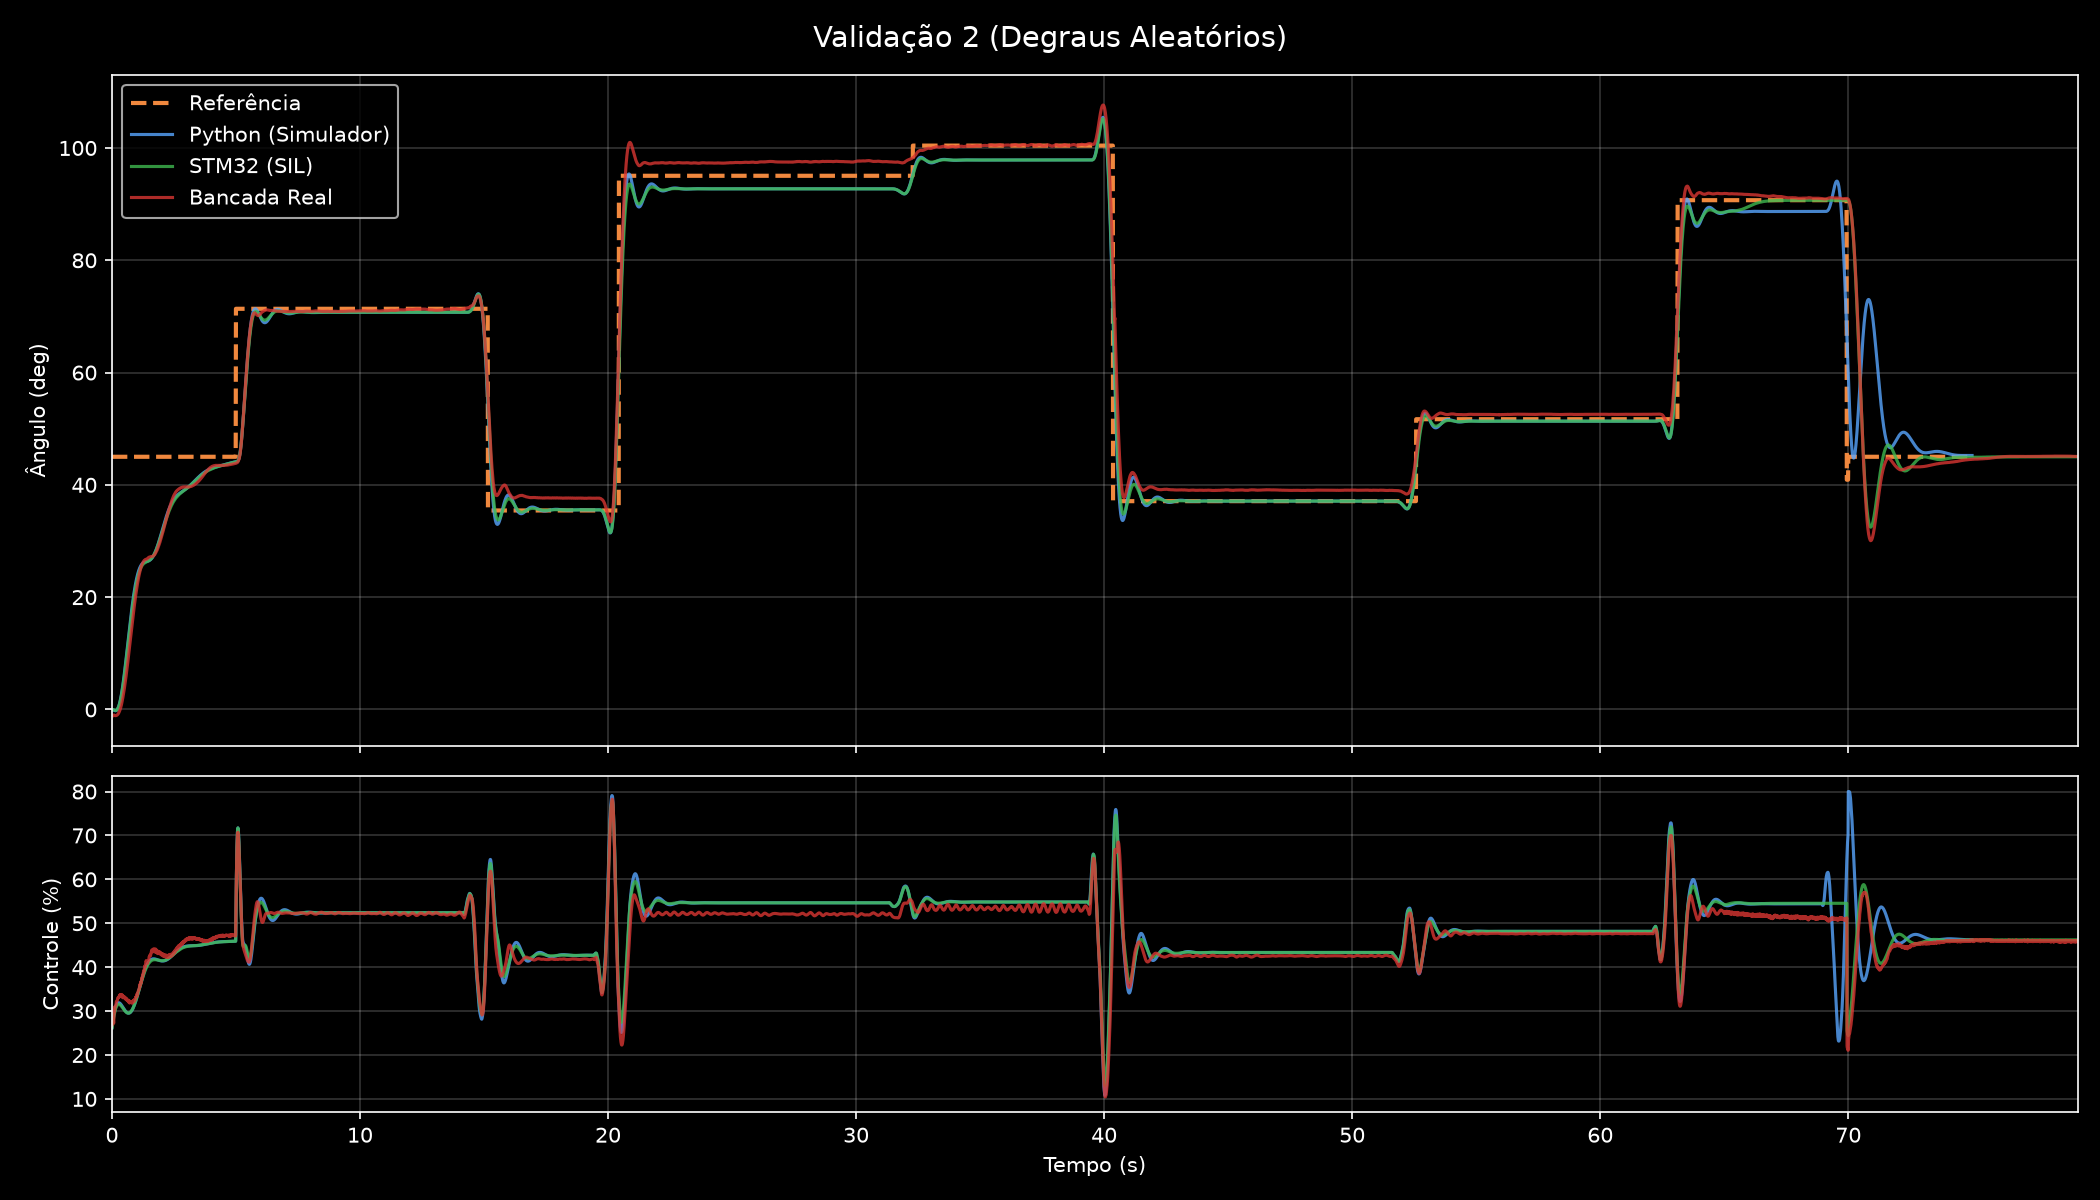
\includegraphics[width=0.95\textwidth]{imagens/comparacao_plot_1.png}
    \caption{Validação 2 (Degraus Aleatórios).}
    \label{fig:val2}
\end{figure}
A transição por degraus aleatórios expôs a métrica mais alta de RMSE (cerca de 4.77$^\circ$ no ambiente real), porém o controle continuou exibindo robustez (\textit{no-windup}) e estabilizou-se rapidamente nas transições sem ocasionar perda do rastreamento, mesmo submetendo o aeropêndulo a inércias pesadas.

\begin{figure}[H]
    \centering
    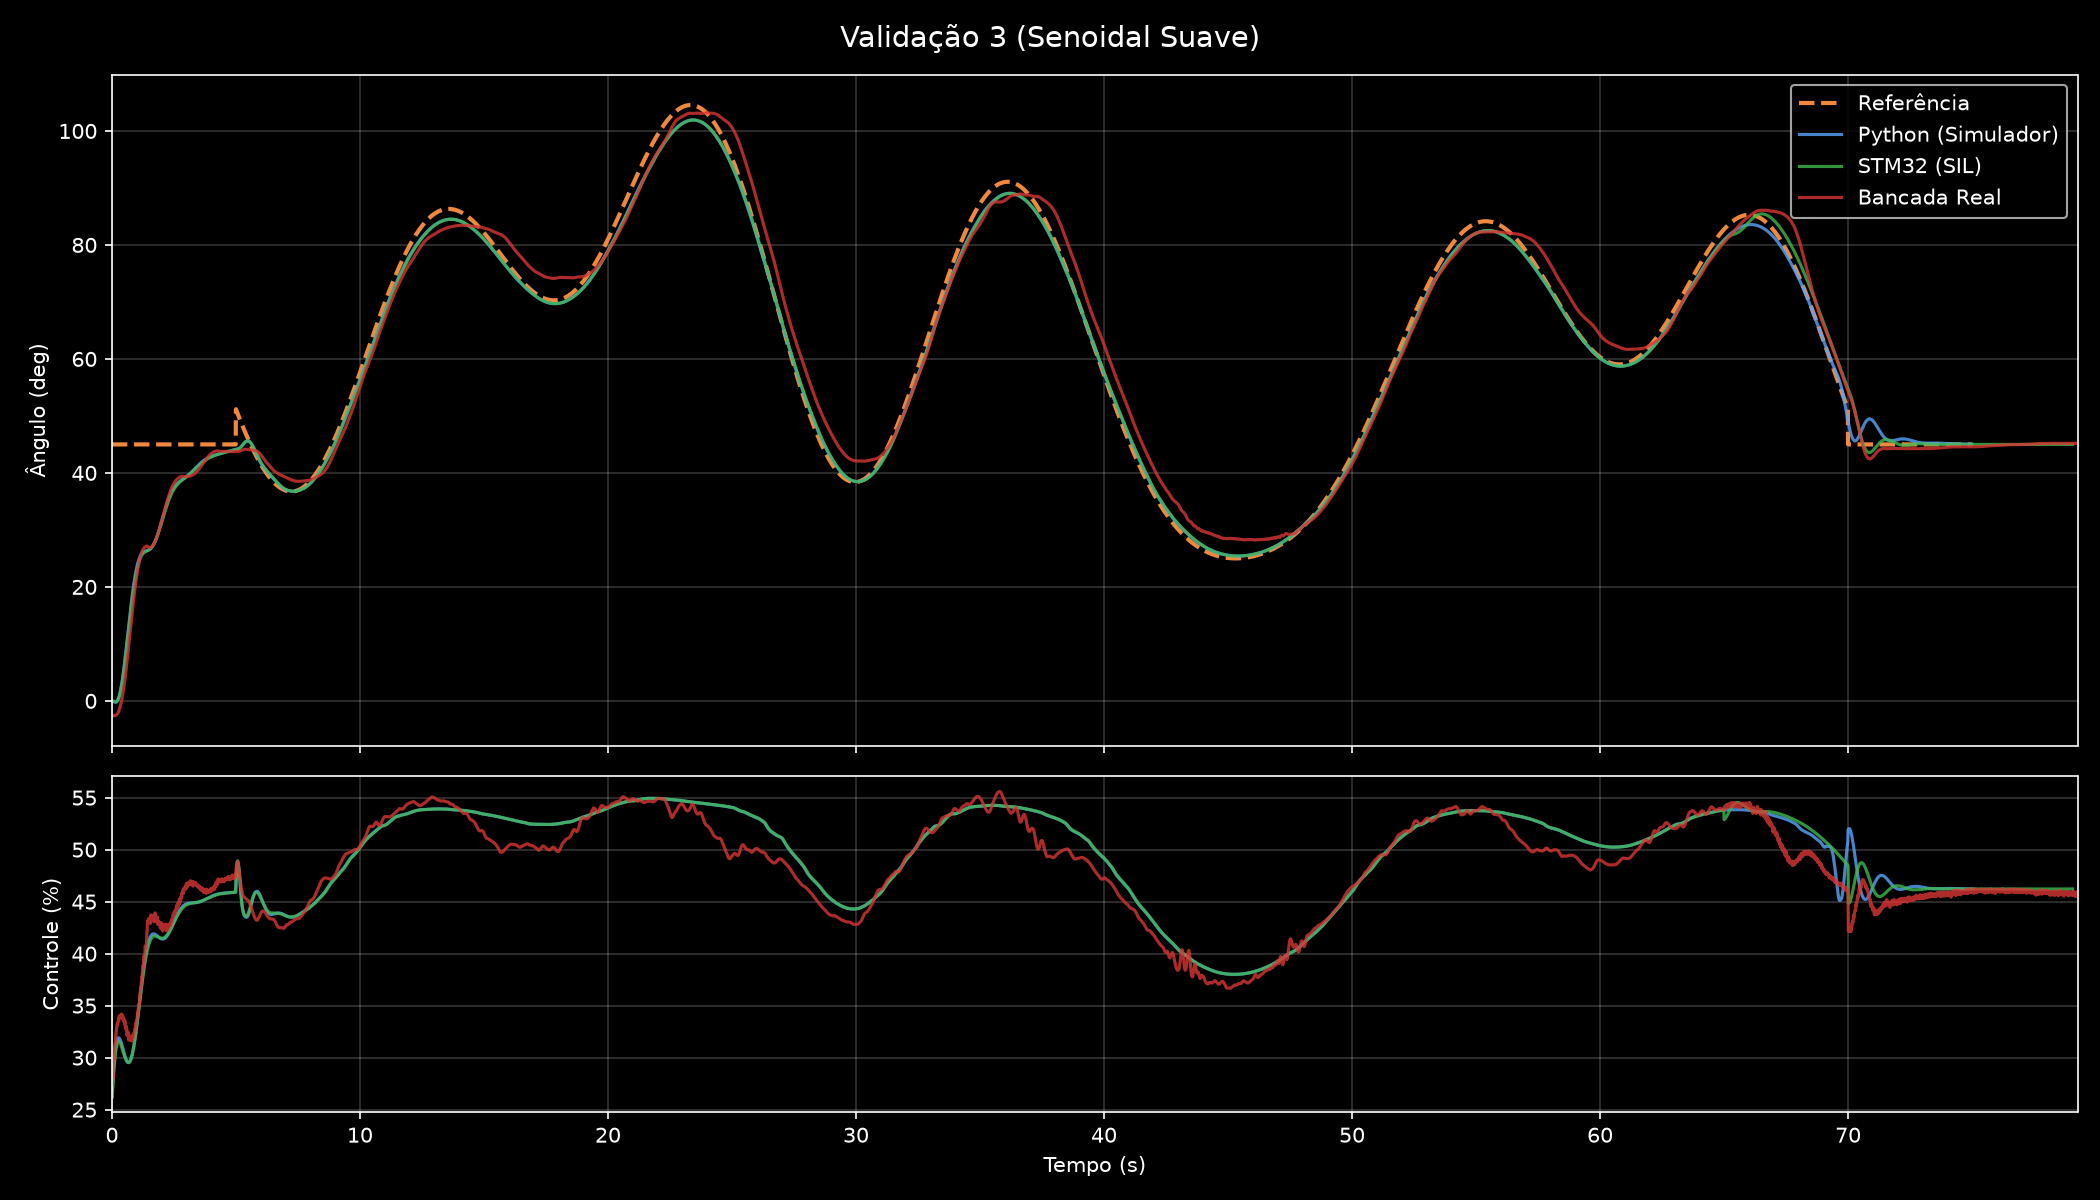
\includegraphics[width=0.95\textwidth]{imagens/comparacao_plot_2.png}
    \caption{Validação 3 (Senoidal Suave).}
    \label{fig:val3}
\end{figure}
Trata-se do comportamento com maior proximidade entre a bancada física e o simulador ideal, provando a extrema eficiência do controle e do mapa do domínio preditivo em regimes permanentes ou referências graduais.

\section{Conclusão e Observações Finais}

O projeto atingiu seu objetivo principal e validou com sucesso a viabilidade de se substituir a elevada demanda computacional da Programação Não-Linear exigida num Controle Preditivo Baseado em Modelo (MPC) pela inferência constante e previsível de uma Rede Neural treinada (\textit{Deep Learning}).

A adoção do CasADi e do treinamento supervisionado via PyTorch confirmou a capacidade do hardware do microcontrolador (STM32) na execução destas políticas sem a perda sensível das garantias de restrição estipuladas \textit{offline}. Comparando as malhas Python, SIL e ambiente Real, os limites de segurança permaneceram controlados, indicando um alto nível de capacidade e generalização do sistema frente ao ruído e às vibrações do arranjo físico e do sensor inercial (IMU).

\end{document}
